\documentclass{beamer}

\usepackage{graphicx}
\usepackage{tabularx}
\usepackage[backend=biber]{biblatex}
\addbibresource{bibliography.bib}


\usetheme{CambridgeUS}


\title{Unsupervised Pretraining of Foundation Models for Medical Imaging}
\author{Scott Chase Waggener}
\date{\today}

\begin{document}

\frame{\titlepage}

\begin{frame}
   \frametitle{Overview}
   \begin{itemize}
        \item Motivation
        \begin{itemize}
            \item Convolutional networks and their limitations
            \item Transformers, strengths and weaknesses
            \item Desired properties of a medical imaging foundation model
        \end{itemize}
        \item Unsupervised Pretraining Methods
        \begin{itemize}
            \item Masked Autoencoder
            \item Contrastive Embedding
            \item Query Box Localization
        \end{itemize}
        \item Results
   \end{itemize}
\end{frame}


\begin{frame}
   \frametitle{Motivation}
   \begin{itemize}
        \item Deep learning models can analyze medical images (such as mammograms) to assist in diagnosis \cite{McKinney2020}
        \item Many such models use convolutional architectures \cite{COGAN201918}, which incorporate a locality prior
        \item Such a prior can accelerate learning, but can also be restrictive
   \end{itemize}
\end{frame}

\begin{frame}
   \frametitle{Motivation}
   \begin{itemize}
        \item Mammographic screenings capture four standard views of the breasts 
        \begin{itemize}
            \item Medio-lateral oblique (MLO)
            \item Cranio-caudal (CC)
            \item MLO and CC views are approximately orthogonal
        \end{itemize}
   \end{itemize}
   \begin{figure}
       \centering
       
\includegraphics[width=0.5\textwidth]{placeholder.jpg}
   \end{figure}
\end{frame}

\begin{frame}
   \frametitle{Motivation}
   \begin{itemize}
        \item The standard views are typically examined together to leverage bilateral symmetry
        \item Reference images are used (when available) to compare to the standard views
        \item Sometimes lesions will appear in multiple views
   \end{itemize}
   \begin{figure}
       \centering
       
\includegraphics[width=0.5\textwidth]{placeholder.jpg}
   \end{figure}
\end{frame}

\begin{frame}
   \frametitle{Motivation}
   A strong mammography model should incorporate all available information:
   \begin{itemize}
        \item Orthogonal nature of MLO and CC views is incompatible with a locality prior
        \item Additional imaging may be available with similar incompatible relationships
        \item Textual information may also be available (medical reports)
   \end{itemize}
   \vspace{1em}
   Similar considerations apply to other medical imaging modalities
\end{frame}

\begin{frame}
   \frametitle{Motivation}
   Objectives to improve mammographic performance:
   \begin{itemize}
        \item Relax the locality prior
        \item Support a variable number of additional context images
        \item Support textual information
   \end{itemize}
   \vspace{1em}
   These objectives will also improve performance on other medical imaging modalities like:
   \begin{itemize}
        \item X-ray
        \item CT
        \item MRI
        \item Ultrasound
   \end{itemize}
\end{frame}

\begin{frame}
   \frametitle{Motivation}
   Vision Transformers (ViTs) can address these objectives:
   \begin{itemize}
        \item Vision Transformers (ViTs) can achieve state-of-the-art results on image classification tasks \cite{dosovitskiy2021image}
        \item Attention is not restricted by a locality prior
        \item Transformers are cardinality invariant
        \item Transformers can support multiple modalities (Med-PaLM2) \cite{singhal2023expertlevel}
   \end{itemize}
   \begin{figure}
       \centering
       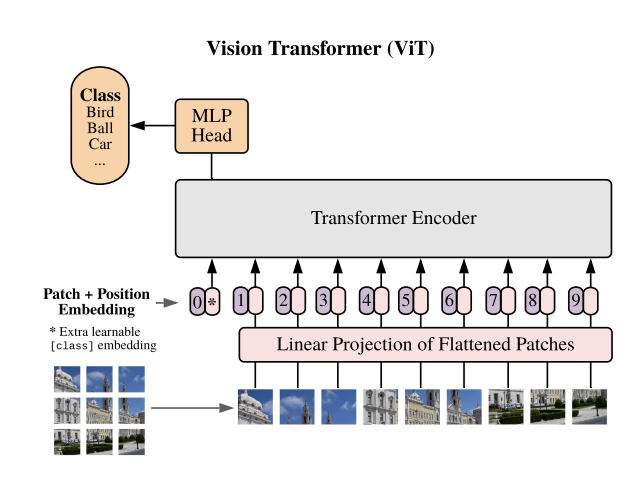
\includegraphics[width=0.5\textwidth]{vit_diagram.png}
   \end{figure}
\end{frame}

\begin{frame}
   \frametitle{Motivation}
   ViTs are not without drawbacks:
   \begin{itemize}
        \item They require a large amount of labeled data (JFT-300M) \cite{dosovitskiy2021image}
        \begin{itemize}
            \item Medical imaging datasets are often small and expensive to label
            \item Thousands of images instead of millions or billions
        \end{itemize}
        \item Or they require clever training methods (DeiT) \cite{pmlr-v139-touvron21a}
        \item Self attention is expensive to compute (quadratic)
        \item Relatively difficult to train from scratch
        \begin{itemize}
            \item Numerical instability
            \item Sensitivity to batch size
            \item Resource intensive
        \end{itemize}
   \end{itemize}
\end{frame}


\begin{frame}
   \frametitle{Masked Autoencoder}
   \begin{itemize}
        \item Follows from masked language modeling (BERT) \cite{devlin2019bert}
        \item Mask a subset of the input patches, regress to the original input
   \end{itemize}
   \begin{figure}
       \centering
       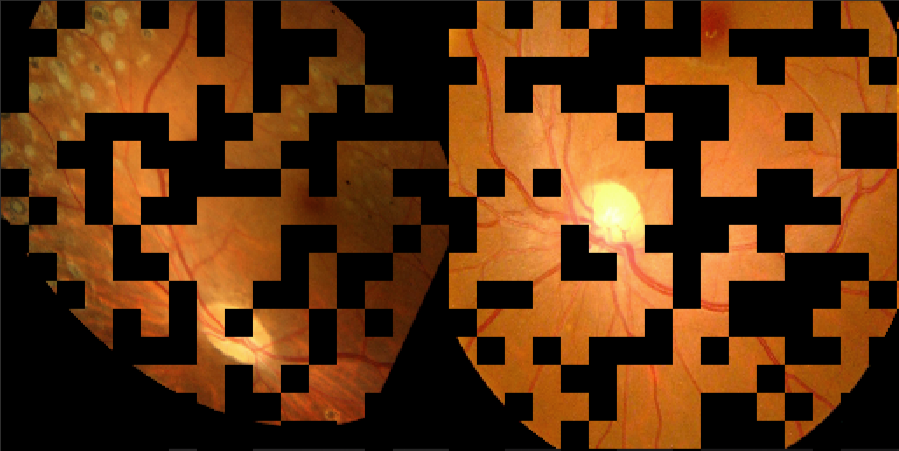
\includegraphics[width=0.5\textwidth]{mae_example.png}
   \end{figure}
\end{frame}

\begin{frame}
   \frametitle{Contrastive Embedding}
   \begin{itemize}
        \item Follows from popular contrastive learning methods (DINO) \cite{caron2021emerging}
        \item Model creates an embedding vector for each image
        \item Embeddings should be similar for augmented versions of the same image
        \item Embeddings should be dissimilar for different images
   \end{itemize}
   \begin{figure}
       \centering
       \begin{minipage}{0.45\textwidth}
           \centering
           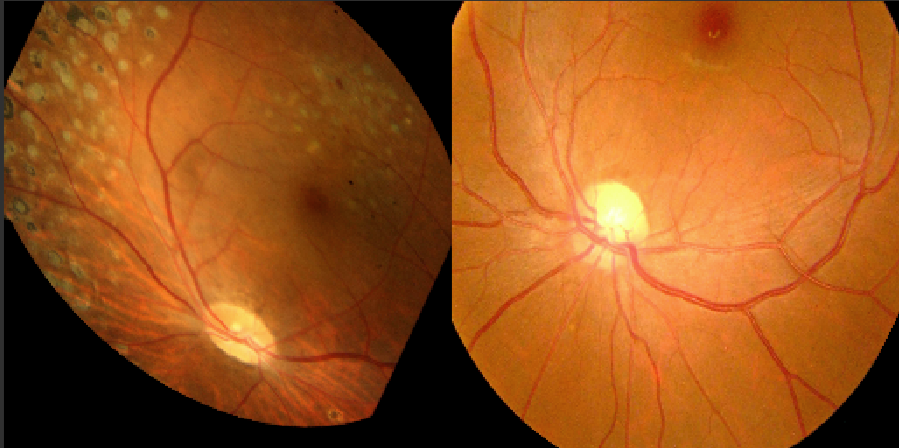
\includegraphics[width=\textwidth]{contrastive_example1.png}
           \caption{Global augmentation}
       \end{minipage}\hfill
       \begin{minipage}{0.45\textwidth}
           \centering
           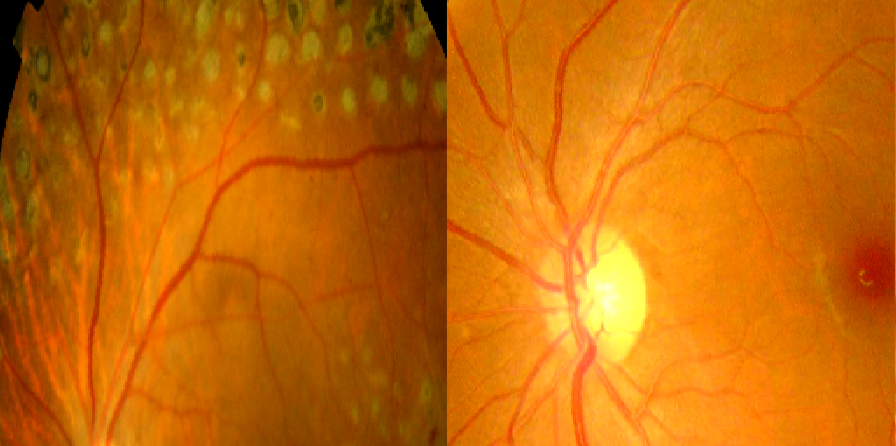
\includegraphics[width=\textwidth]{contrastive_example2.png}
           \caption{Local augmentation}
       \end{minipage}
   \end{figure}
\end{frame}

\begin{frame}
   \frametitle{Query Box Localization}
   \begin{itemize}
        \item Inspired by UP-DETR, a pretraining method for detection models \cite{Dai_2022}
        \item Regions of interest are randomly selected and augmented
        \item Given the original image and the augmented image, the model should predict the bounding box of the region of interest
   \end{itemize}
   \begin{figure}
       \centering
       \begin{minipage}{0.45\textwidth}
           \centering
           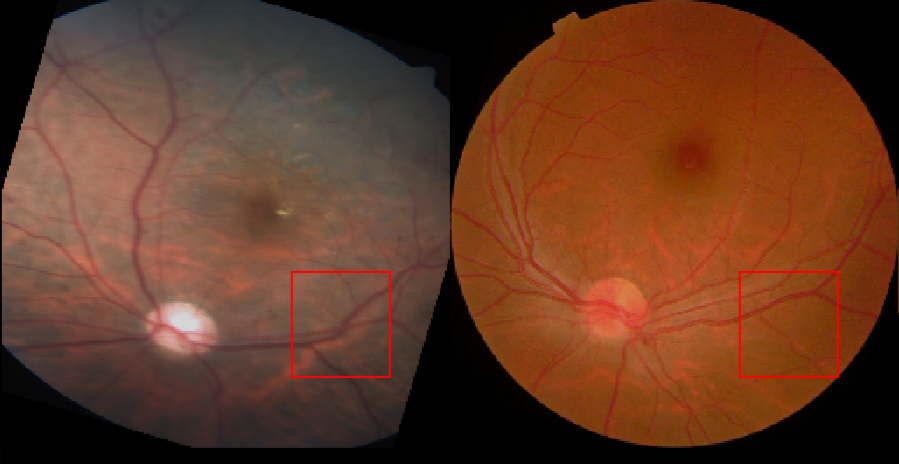
\includegraphics[width=\textwidth]{query_box_1.png}
           \caption{Original image}
       \end{minipage}\hfill
       \begin{minipage}{0.45\textwidth}
           \centering
           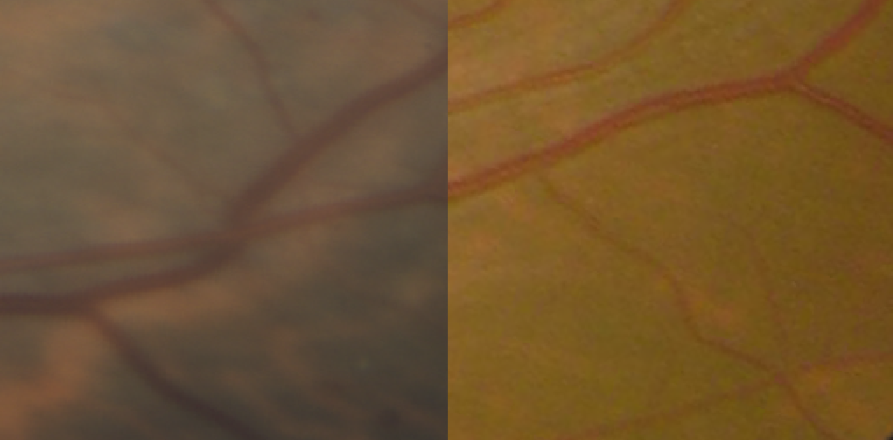
\includegraphics[width=\textwidth]{query_box_2.png}
           \caption{Augmented ROIs}
       \end{minipage}
   \end{figure}
\end{frame}

\begin{frame}
   \frametitle{Methods}
   Architecture:
   \begin{itemize}
        \item Inspired by ViTDet \cite{li2022exploring}
        \item Standard patch embedding with log-spaced sinusoidal position embeddings
        \item Window attention without shifting
        \item Global attention at periodic intervals
   \end{itemize}
   \vspace{1em}
   Training:
   \begin{itemize}
        \item One or more of the pretraining methods are incorporated into the training process
        \item Tasks are cyclically sampled at each minibatch
   \end{itemize}
\end{frame}

\begin{frame}[shrink=30]
   \frametitle{References}
   \printbibliography
\end{frame}


\end{document}
